\section{Problema 3: La comunidad del anillo}

\subsection{Introducci\'on}

Nuestra empresa, AlgoNET, se dedica principalmente a brindar soluciones algor\'itmicas para problemas de redes y en esta ocasi\'on nos enfrentamos al siguiente desaf\'io.
\\
\\
Nuestro cliente quiere ofrecer un servicio particular sobre de una red existente de computadoras. La red consta actualmente de conexiones entre algunos pares de equipos y cada enlace tiene un costo de utilizaci\'on determinado.
\\
\\
Se pretende seleccionar algunas de estas computadoras para utilizar como servidores formando un backbone con topolog\'ia de anillo (cada servidor tiene un enlace directo con exactamente otros 2, uno de entrada y otro de salida).
Adicionalmente se requiere que todas las dem\'as computadoras puedan tener acceso a los servidores del anillo, ya sea por un enlace directo o pasando a traves de otros equipos en el camino.
\\
\\
Se nos pid\'io implementar un algoritmo con complejidad estrictamente menor a $O((\#computadoras)^3)$ que nos permita saber que conexiones utilizar formar el anillo y cuales emplear para conectar el resto de los equipos, de manera de minimizar el costo incurrido por el uso de los enlaces.


\subsubsection{Ejemplo pr\'actico:}

\begin{figure}[h]
  \centering
    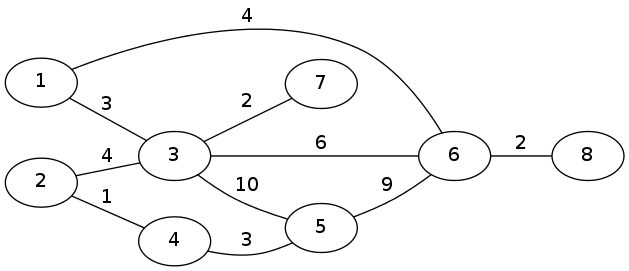
\includegraphics[scale=0.45]{ej3/intro1.png}
  \caption{Ejemplo de red con 8 computadores y 10 enlaces con costos asociados}
  \label{fig:ejemplo}
\end{figure}

\begin{figure}[h]
  \centering
    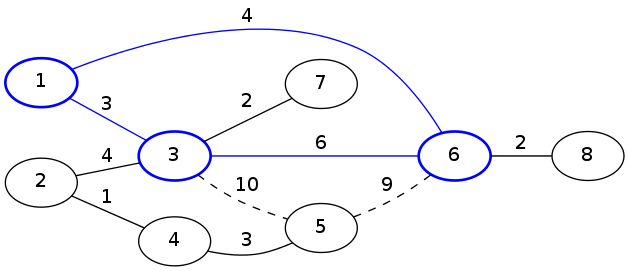
\includegraphics[scale=0.45]{ej3/intro2.png}
  \caption{Soluci\'on del ejemplo}
  \label{fig:ejemplo}
\end{figure}
\begin{itemize}
\item Los equipos 1, 3 y 6 forman el anillo de servidores.
\item Los enlaces (5,6) y (3,5) no son utilizados.
\item El resto de las computadoras se encuentran conectadoa con el anillo ya sea directamente como el equipo 8 con el servidor 6 o indirectamente como el computador 4 que se conecta con el servidor 3 pasando primero por el equipo 2.
\item Costo total de los enlaces utilizados = 25.
\end{itemize}

\subsection{Idea General}

Decidimos modelar el problema utilizando teor\'ia de grafos.
\begin{itemize}
\item Cada nodo representar\'a una computadora de la red.
\item Dos nodos ser\'an adyacentes si y solo si existe un enlace entre los 2 equipos.
\item Ser\'a un grafo pesado, el peso de una arista representa el costo de utilizaci\'on del enlace.
\end{itemize}

Dividiremos el problema en dos partes:
\begin{itemize}
\item Primero dejaremos de lado la parte de formar un anillo y conectaremos todas las computadoras minimizando el costo incurrido en los enlaces, es decir, buscaremos un arbol generador minimo sobre el grafo.
\item Luego, buscaremos la arista de menor peso que no forme parte del AGM y se la agregaremos. De esta manera formaremos un ciclo y ese ser\'a nuestro ''anillo''.
\end{itemize}

\subsection{Desarrollo}

La implementaci\'on fue hecha en codigo $c++$.
\\
\\
Para buscar el AGM implementamos un algoritmo basado en PRIM

\LinesNumbered
\begin{algorithm}[H]
\DontPrintSemicolon
\Begin{
	\If{\# Aristas $<$ \# Nodos}{
		No existe soluci\'on\;
		\textbf{return} 1\;
	}

	cola = heap con punteros a todos los nodos del grafo\;
	raiz$\rightarrow$distancia = 0\;

	\While{!esta\_vacia(cola)}{
		u = extraer\_minimo(cola)\;
		\If{u$\rightarrow$distancia == INF}{
			Sin Soluci\'on, no es conexo\; 
			\textbf{return} 1\;
		}
		costoTotal += u$\rightarrow$distancia\;
		Anotamos la arista que une u con u$\rightarrow$Padre como parte del AGM\;
		agendamos u como ya recorrido\;
		\For {v $\in$ adyacentes de u}{
			\If {!recorrido(v) \&\& v$\rightarrow$distancia $>$ peso(u,v)}{
				v$\rightarrow$padre = u\;
        v$\rightarrow$distancia = peso(u,v)\;
			}
		}
	}
	\textbf{return} 0\;
}
\caption{\textbf{buscar\_AGM()} \label{buscar\_AGM }}
\end{algorithm}

Donde
\begin{itemize}
\item $raiz$ es el Nodo numero 1 del grafo.
\item $distancia$ se encuentra inicializada en INF para todos los nodos.
\item El $padre$ de cada nodo se encuentra inicializado en NULL.
\item El heap esta ordenado por menor distancia.
\item En $costoTotal$ guardamos el costo total de la utilizaci\'on de los enlaces incluidos en el AGM.
\end{itemize}

Una vez que tenemos generado en AGM, procedemos a buscar la arista de menor peso no incluida en el AGM para formar un ciclo, de la siguiente manera:

\LinesNumbered
\begin{algorithm}[H]
\DontPrintSemicolon
\Begin{
	sort 'aristas' de menor a mayor peso\;

    \For {e $\in$ aristas}{
    	\If{e $\not\in$ AGM}{
            costoTotal += peso(e)\;
            arista\_extra = e\;
            break\;
    	}
    }

    \For {x$_1$, x$_2$ $\in$ nodos incidentes a $arista\_extra$}
    {        
        \While{x$_1$ $\neq$ raiz \&\& x$_1$ $\neq$ x$_2$ }
        {
        	Anotamos $x_1$ como parte del anillo\;
            x$_1$ = x$_1$ $\rightarrow$padre\;
        }
    }

    \For {k $\in$ nodos}
    {
        \If {k $\neq$ raiz}
        {
            \If {k esta anotado como parte del anillo}
            {
                anillo.push\_back(arista que une a k con su padre)\;
            }
            \Else{
                resto.push\_back(arista que une a k con su padre)\;
            }
        }
          
    }
}
\caption{\textbf{formar\_anillo()} \label{formar\_anillo }}
\end{algorithm}







\subsection{Demostraci\'on de correctitud} 


Primero notemos que la solución óptima posee un solo circuito o “anillo”, ya que si posee más de uno puedo eliminar uno de ellos, pues sea C uno de ellos donde C = $v_1$, $v_2$, …, $v_i$, $v_1$ con 2 $\leq$ i $<$ n puedo eliminar la arista que une $v_i$ con $v_1$ cuyo peso es $>$ 0 obteniendo una solución del problema de peso menor que la óptima por lo que es absurdo. \\




Queremos ver que la solucion que da nuestro algoritmo es optima, es decir que cualquier solucion optima es un AGM + la arista menos pesada fuera del AGM. Por lo que vamos a ver que: \\


\begin{itemize}


	\item	Dado A una solucion optima, sea “e” el eje más pesado del único circuito que posee, queremos ver que A-\{e\} es un AGM.\\


	\textbf{Demostración:} \\
	Sea T AGM $\Longrightarrow$ costo(T) $\leq$ costo(A-\{e\}) ya que A-\{e\} es un AG hasta el momento (es un grafo acíclico ya que sacamos una arista del único ciclo que poseía, y es conexo que contiene a todos los nodos porque la solución tiene que contener a todos los nodos, existiendo un camino entre todos ellos hacia el anillo, por lo tanto, es un árbol generador).\\
	Si e no está en T, ya está, ya que si A fuera de mayor peso que T rearmaría la solución como T+\{e\}, la cual posee un único ciclo obteniendo una solución de menor peso, lo que es absurdo porque A era óptima. Entonces costo(A-\{e\}) $\leq$ costo(T) y por lo tanto A-\{e\} es un AGM.\\
	Caso contrario tomo un eje e’ que no pertenece a T del circuito que contiene a “e” en A (existe ya que como e pertenece a T, si todas las demás aristas también pertenecieran a T, entonces T tendría un ciclo, y esto es ABS!). Luego T+\{e'\} tiene un único circuito simple. \\
	 Si el costo de A fuera $>$ que costo(T+\{e'\}), utilizaría a T+\{e'\} como solución y sería mejor que la óptima, que es ABS! $\Rightarrow$ costo(A) $\leq$ costo(T+\{e'\}) por lo que podemos llegar a que: \\
	
	Costo(A) $\leq$ costo(T)+costo(\{e'\}) $\leq$ costo(T)+costo(e) ya que “e” es la arista más pesada del ciclo en A y e’ pertenecía a ese ciclo en A. Resultando en costo(A-\{e\}) $\leq$ costo(T) como queríamos demostrar. \\
	
	




	\item	Ahora vamos a demostrar que si tomo un AGM T, entonces el eje e’ de peso mínimo del grafo que no esta en T, entonces peso(e’) $\leq$ peso(e)\\
	
Para esto vamos a renombrar ciertas cosas:

\begin{itemize}
	\item	T = el AGM del óptimo = A-\{e'\}
	\item	T’ = un AGM
	\item	e = eje mas pesado del ciclo en la solución óptima
	\item	e’ = eje más liviano fuera de T’
\end{itemize}

	
	\textbf{Demostración:} \\
	Sabemos que existe un eje e’’ de C que no está en T’ ya que T’ es a cíclico. Con esto podemos derivar que costo(e’) $\leq$ costo(e’’) ya que e’ y e’’ son ejes que están fuera de T’ y e’ era la más liviana. Y en particular costo(e’’) $\leq$ costo(e) ya que e era el eje más pesado del ciclo C. Con lo que queda que costo(e’) $\leq$ costo(e) como queríamos demostrar

\end{itemize}


\newpage
\subsection{Complejidad}


buscar\_AGM es basicamente un algoritmo de PRIM, el mismo tiene complejidad temporal O($n^2$).
\\
Analizemos entonces la complejidad de formar el anillo:

\begin{codebox}
\Procname{$\proc{\textbf{formar\_Anillo()\{}}$}
\li \ \ sort(aristas.begin(), aristas.end());   \RComment{O(M*$\log{M}$)}
\li \ \ pair$<$Nodo*, Nodo*$>$ arista\_extra; \RComment{O(1)}
\li \ \ for (unsigned int i = 0; i $<$ aristas.size(); i++) \RComment{O(M)}
\li \ \ \{
\li \ \ \ \ if(aristas[i].second.first$\rightarrow$arista\_en\_AGM[aristas[i].second.second$\rightarrow$numero] == 0) \RComment{O(1)}
\li \ \ \ \ \{\ \ 
\li \ \ \ \ \ \ C += aristas[i].first;  \RComment{O(1)}
\li \ \ \ \ \ \ arista\_extra = aristas[i].second;  \RComment{O(1)}
\li \ \ \ \ \ \ break;
\li \ \ \ \ \}
\li \ \ \}
\li \ \ Nodo * a = arista\_extra.first; \RComment{O(1)}
\li \ \ Nodo * b = arista\_extra.second;  \RComment{O(1)}
\li \ \ for (int i = 0; i $<$ 2; i++) \RComment{O(1)}
\li \ \ \{\ \ \ \ 
\li \ \ \ \ while(a $\neq$ NULL \&\& a $\neq$ b)    \RComment{O(N)}
\li \ \ \ \ \{
\li \ \ \ \ \ \ a$\rightarrow$en\_anillo = true;  \RComment{O(1)}
\li \ \ \ \ \ \ a = a$\rightarrow$padre;          \RComment{O(1)}
\li \ \ \ \ \}
\li \ \ \ \ a = arista\_extra.second;             \RComment{O(1)}
\li \ \ \ \ b = arista\_extra.first;              \RComment{O(1)}
\li \ \ \}
\li \ \ anillo.push\_back(arista\_extra);       \RComment{O(1)}
\li \ \ for (int i = 1; i $\leq$ N; i++)      \RComment{O(N)}
\li \ \ \{
\li \ \ \ \ Nodo* k = &nodos[i];          \RComment{O(1)}
\li \ \ \ \ if (k$\rightarrow$padre $\neq$ NULL)      \RComment{O(1)}
\li \ \ \ \ \{
\li \ \ \ \ \ \ if (k$\rightarrow$en\_anillo)   \RComment{O(1)}
\li \ \ \ \ \ \ \{
\li \ \ \ \ \ \ \ \ anillo.push\_back(make\_pair(k, k$\rightarrow$padre));    \RComment{O(1)}
\li \ \ \ \ \ \ \}
\li \ \ \ \ \ \ else
\li \ \ \ \ \ \ \ \ resto.push\_back(make\_pair(k, k$\rightarrow$padre));     \RComment{O(1)}
\li \ \ \ \ \}
\li \ \ \}
\li \}
\end{codebox}

\begin{itemize}
\item La funci\'on de sort ordena todas las aristas se\'gun su peso, tiene complejidad O(M*$\log{M}$) con M = \# de aristas.
\item El for de la linea 3, itera sobre todas las aristas (M) hasta encontrar una que no este usada en el AGM. Luego tiene complejidad O(M).
\item El for de la linea 14, forma el anillo iterando los padres de cada uno de los nodos incidentes a la arista\_extra. A lo sumo iterar\'a  todos los nodos del grafo (en el caso en que el grafo sea un C$_n$). Luego tiene complejidad O($N$)
\item El for de la linea 25 itera todos los nodos del grafo, chequeando en O(1) si perteneces al anillo o no, y los va separando. La complejidad nos queda O(N).
\end{itemize}
\newpage
Luego, la complejidad total nos queda:
$$O(M*\log{M})+O(M)+O(N)+O(N) = O(M*\log{M}) \leq O(N^2*\log{N^2}) < N^3$$




\subsection{Testing}

\subsubsection{Conexo sin ciclos}

\begin{figure}[h]
  \centering
    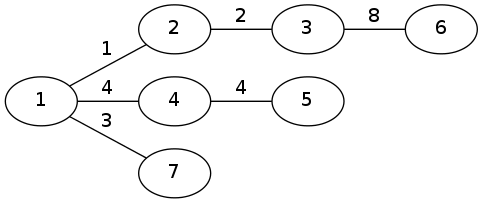
\includegraphics[scale=0.45]{ej3/caso0-1.png}
  \caption{Grafo conexo sin ciclos}
  \label{fig:ejemplo}
\end{figure}
~
\\
La entrada en s\'i es un arbol, al no tener ciclos no podremos encontrar un anillo de servidores.
El algoritmo deja de ejecutar al darse cuenta que M $<$ N y devuelve $-1$.

\subsubsection{No conexo con ciclos}
\begin{figure}[h]
  \centering
    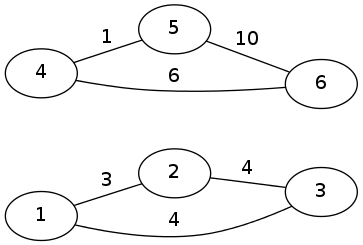
\includegraphics[scale=0.45]{ej3/caso2-1.png}
  \caption{Grafo no conexo con ciclos}
  \label{fig:ejemplo}
\end{figure}
~
\\
Si bien M $\geq$ N, al ser el grafo no conexo, no podremos encontrar un camino de enlaces de cada computadora a un servidor.\\
El algoritmo buscar\_AGM devolver\'a $-1$ al extraer del heap un nodo con distancia == Infinito.

\subsubsection{Cn}
\begin{figure}[h]
  \centering
    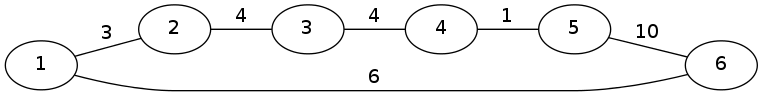
\includegraphics[scale=0.45]{ej3/caso1-1.png}
  \caption{Grafo C$_6$}
  \label{fig:ejemplo}
\end{figure}
~
\\
Caso borde donde todos equipos deben ser utilizados como servidores para que haya soluci\'on
\begin{figure}[h]
  \centering
    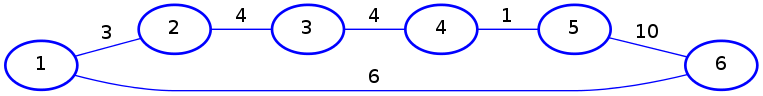
\includegraphics[scale=0.45]{ej3/caso1-2.png}
  \caption{Salida grafo C$_6$}
  \label{fig:ejemplo}
\end{figure}



\newpage
\subsubsection{Todos los enlaces con el mismo coste}
\begin{figure}[h]
  \centering
    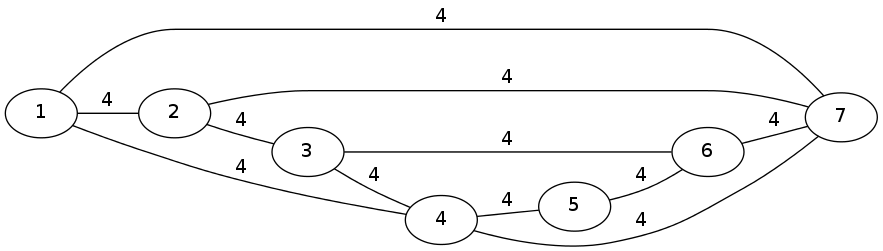
\includegraphics[scale=0.45]{ej3/caso3-1.png}
  \caption{Todos los enlaces con el mismo coste}
  \label{fig:ejemplo}
\end{figure}
~
\\
Caso borde donde todos los enlaces tienen el mismo costo de utilizaci\'on.\\
Todas las combinaciones de N aristas son soluciones \'optimas.
\begin{figure}[h]
  \centering
    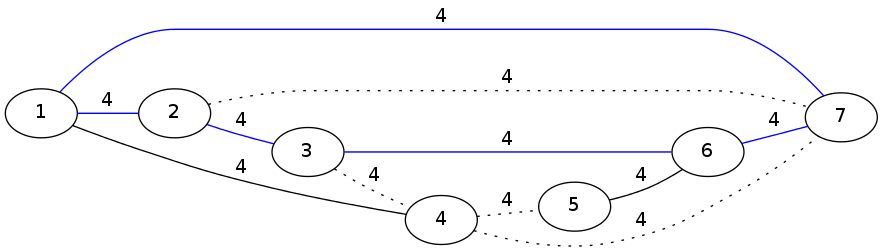
\includegraphics[scale=0.45]{ej3/caso3-2.png}
  \caption{Salida todos los enlaces con el mismo coste}
  \label{fig:ejemplo}
\end{figure}
\\
~
\newpage
\subsubsection{Caso general}
\begin{figure}[h]
  \centering
    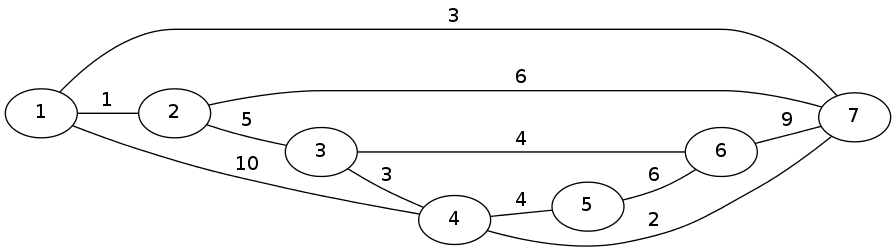
\includegraphics[scale=0.45]{ej3/caso4-1.png}
  \caption{Ejemplo de red con 8 computadores y 10 enlaces con costos asociados}
  \label{fig:ejemplo}
\end{figure}
~
\\
Un caso m\'as general, el mismo grafo que en el punto anterior pero costos de enlace variables.
\begin{figure}[h]
  \centering
    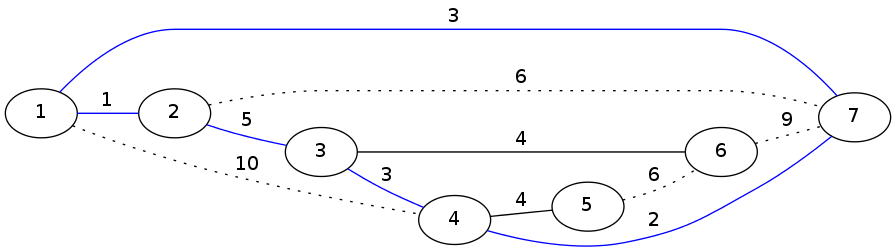
\includegraphics[scale=0.45]{ej3/caso4-2.png}
  \caption{Ejemplo de red con 8 computadores y 10 enlaces con costos asociados}
  \label{fig:ejemplo}
\end{figure}


\subsection{Experimentación}
Una vez hecho el análisis de la complejidad teórica, realizamos experimentos con el fin de contrastar los resultados empíricos y comprobar que el algoritmo implementado efectivamente tendrá una complejidad temporal de O(n$^{2}$).\\
Para los siguientes experimentos  se toman una distribución discreta uniforme entre 1 y 100 que se utilizan como valor para el costo de un enlace.

El grueso de nuestra experimentación va a estar dado si el grafo es denso o poco denso para un n fijo.
Para reducir los posibles errores de medición y evitar que los resultados se vean alterados por entradas de peor o mejor caso sesgando los resultados, se decidió tomar una cantidad fija de 220 instancias generadas y tomar el promedio. En el siguiente grafico se pueden observar los resultados:

\begin{figure}[H]
                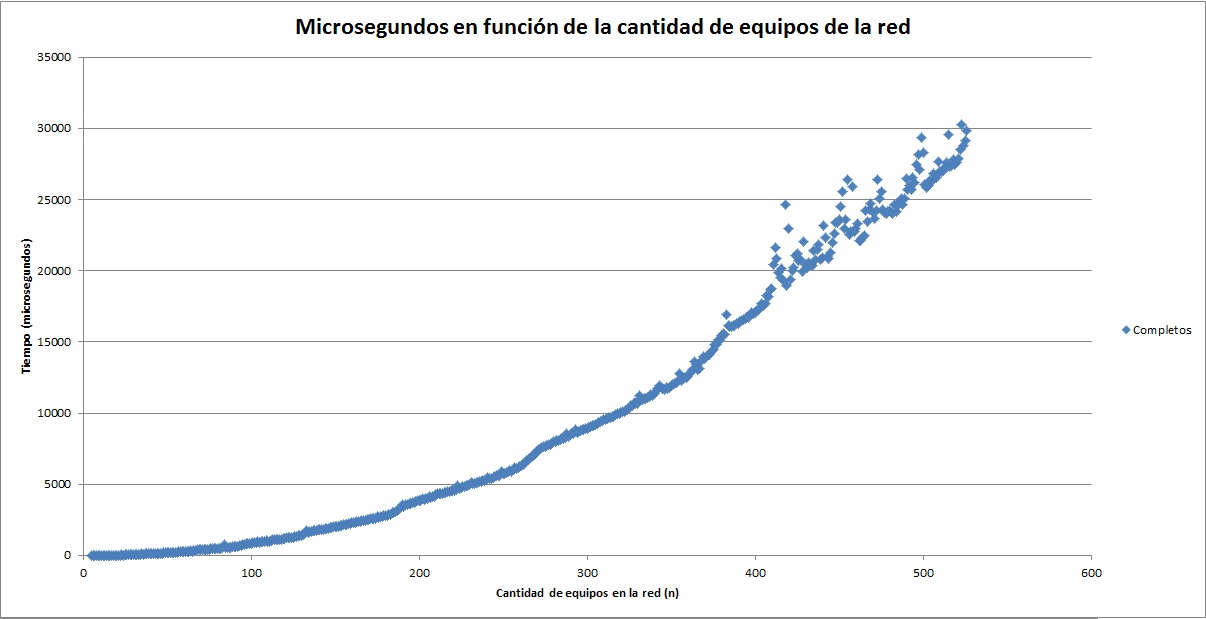
\includegraphics[scale=0.6]{ej3/comple}
                \caption{}
                \label{fig:exp2}
\end{figure} 



\begin{figure}[H]
                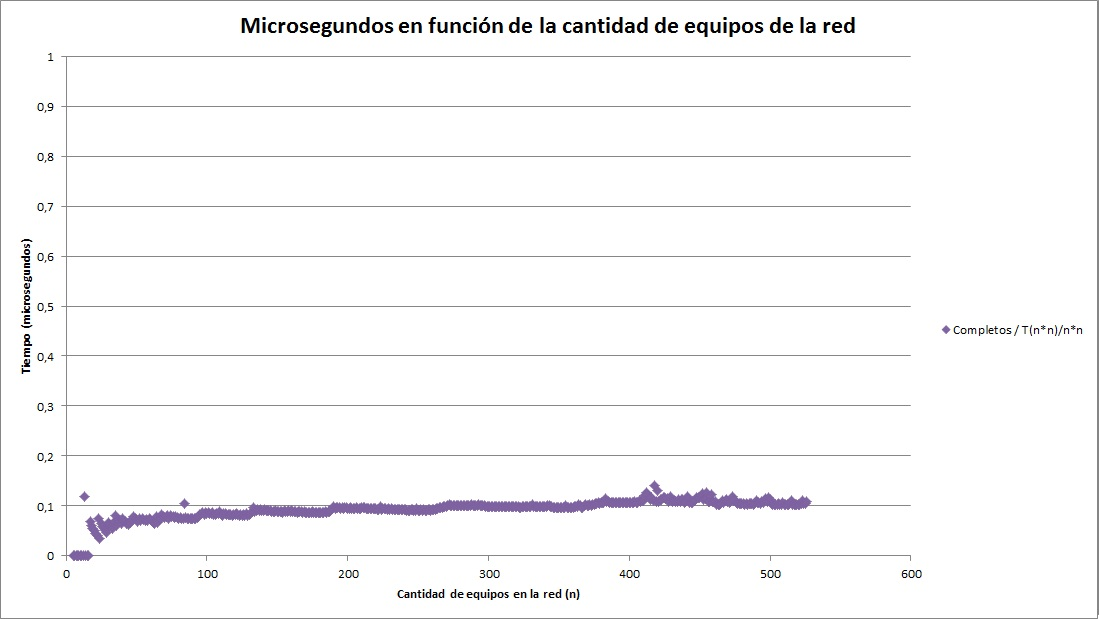
\includegraphics[scale=0.6]{ej3/compleConst}
                \caption{}
                \label{fig:exp2}
\end{figure}


\begin{figure}[H]
                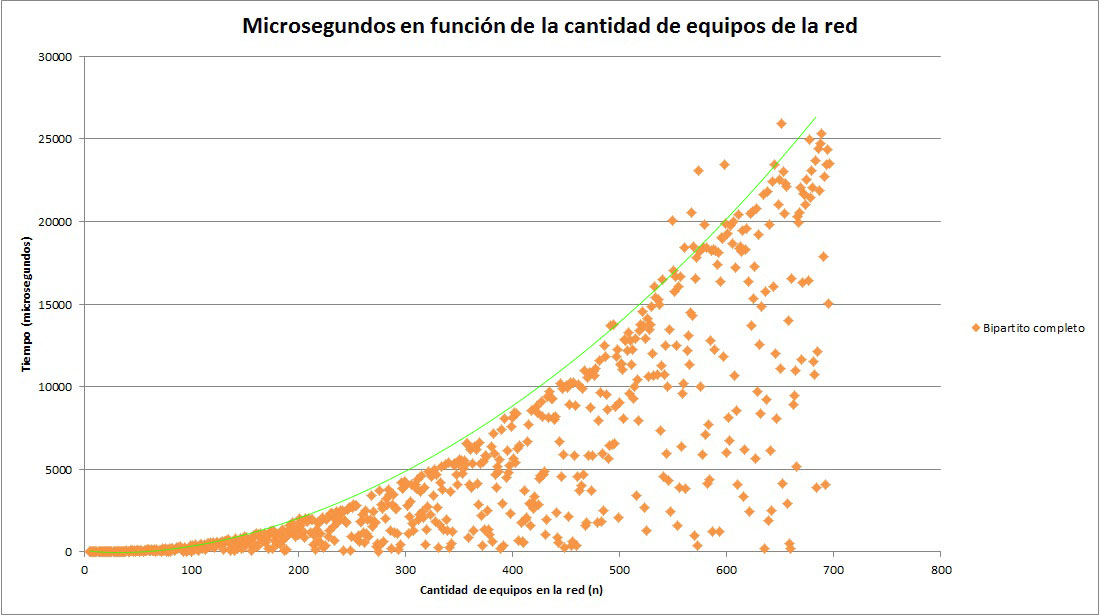
\includegraphics[scale=0.4]{ej3/bPartCom}
                \caption{}
                \label{fig:exp2}
\end{figure} 



\begin{figure}[H]
                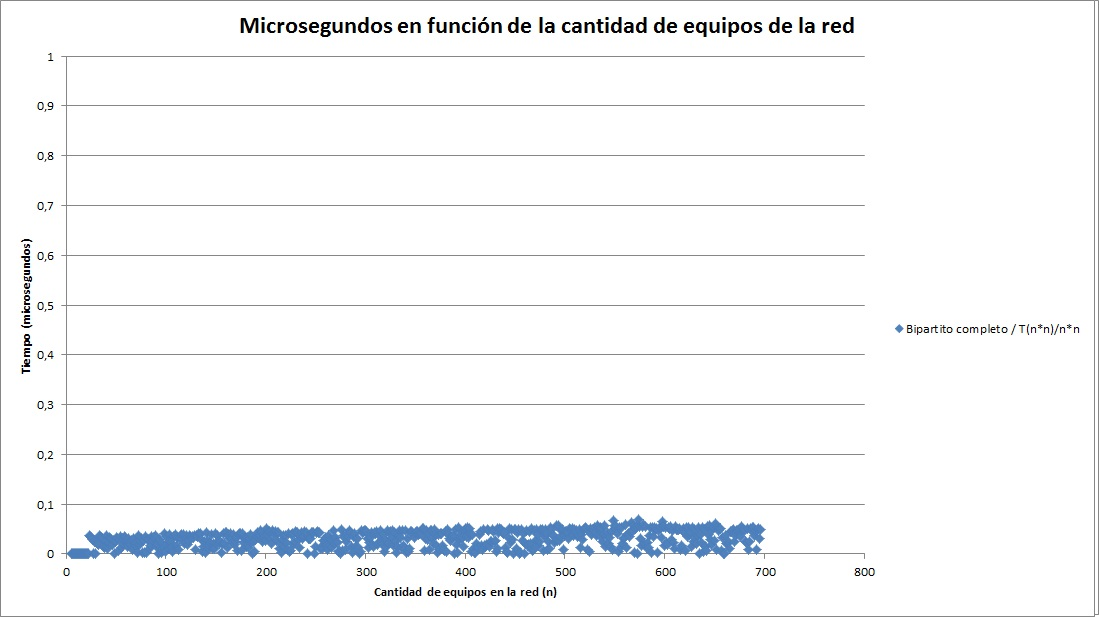
\includegraphics[scale=0.6]{ej3/bPartComConst}
                \caption{}
                \label{fig:exp2}
\end{figure}                 

\begin{figure}[H]
                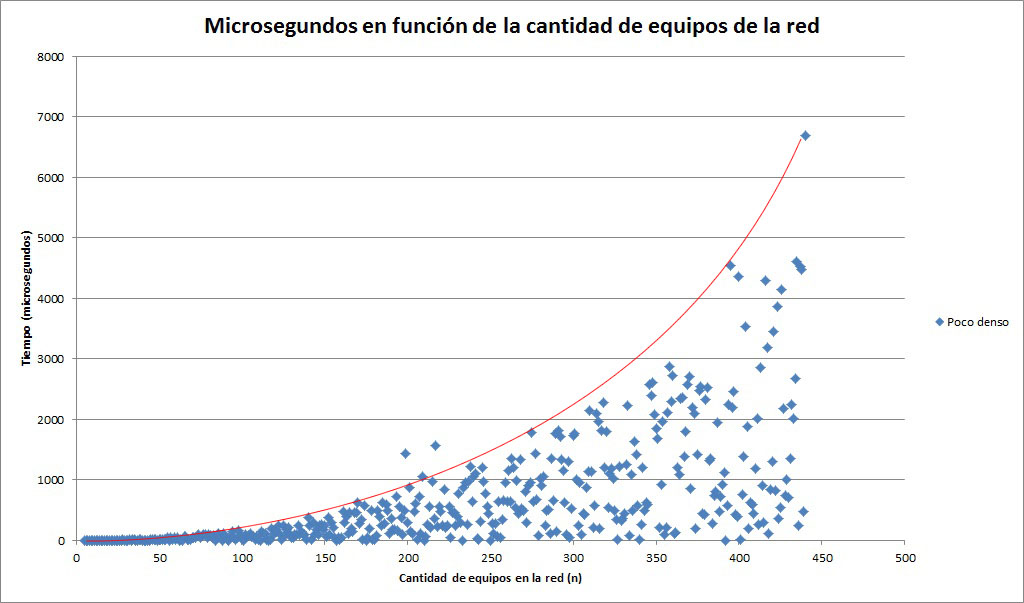
\includegraphics[scale=0.4]{ej3/pDenso}
                \caption{}
                \label{fig:exp2}
\end{figure} 



\begin{figure}[H]
                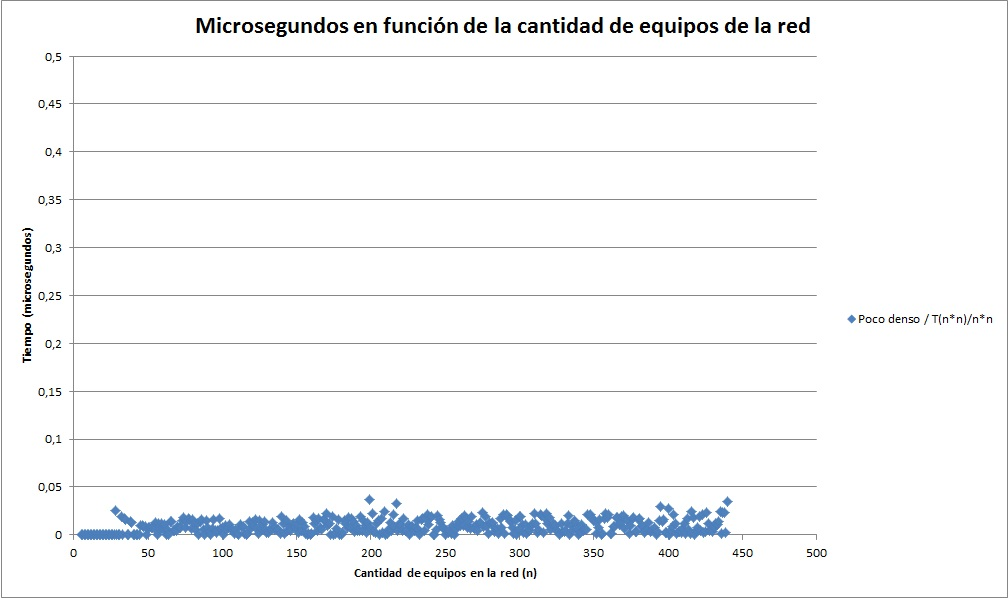
\includegraphics[scale=0.6]{ej3/pDensoConst}
                \caption{}
                \label{fig:exp2}
\end{figure}  

En estos graficos podemos corroborar que efectivamente la complejidad es $O(n^2)$. Ahora vamos a comparar dichas configuraciones de grafos para ver si efectivamente la densidad afecta en la complejidad, no a tal punto de hacerla crecer mas que $n^2$ pero de tener una constante mas alta.


\begin{figure}[H]
                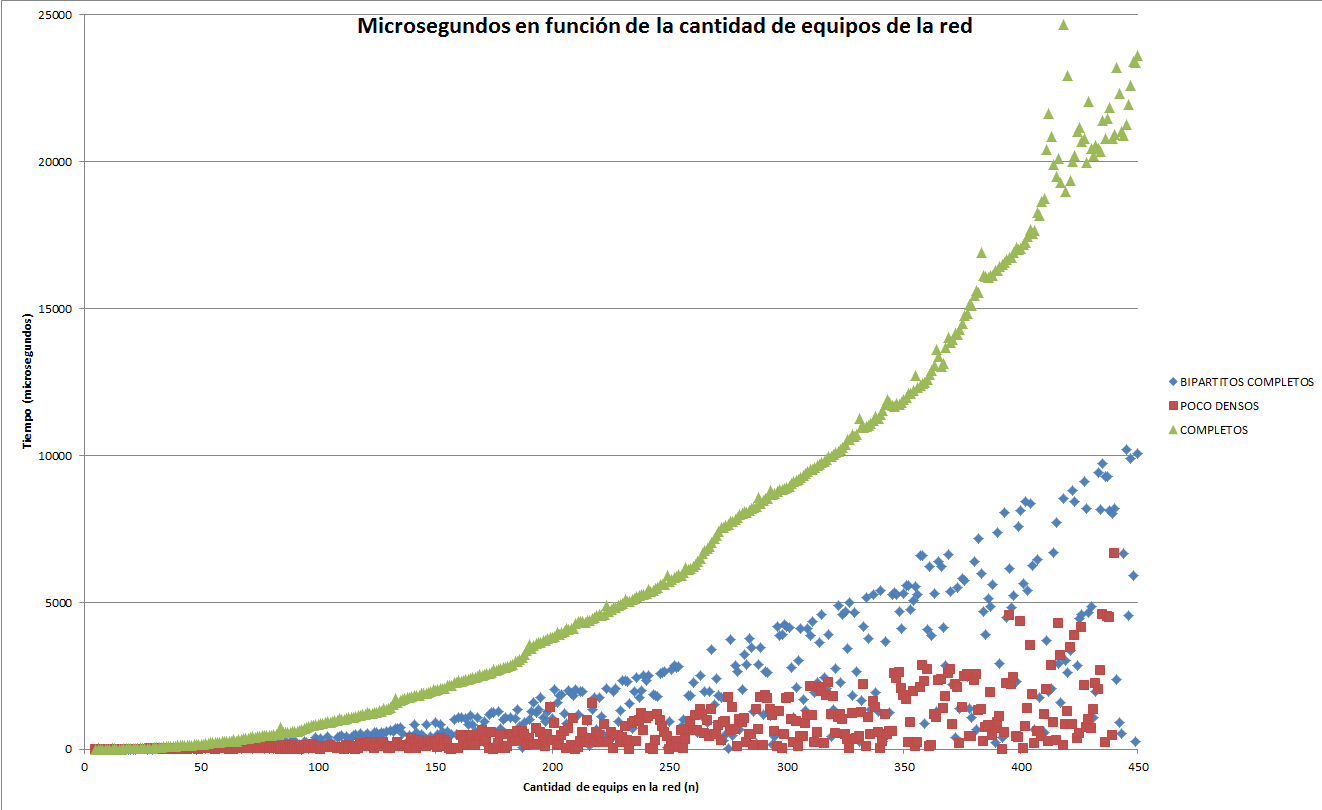
\includegraphics[scale=0.5]{ej3/Comparaciones}
                \caption{}
                \label{fig:exp22}
\end{figure}

Como el grueso de nuestro algoritmo se basa en buscar un AGM entonces los grafos mas densos van a tener mas cantidad de aristas, haciendo que el algoritmo tarde mas en encontrarlo. Esto se corrobora con los gráficos, como en el gráfico \ref{fig:exp22} que es notable la diferencia de tiempos entre el mas denso y el menos denso.\\
Podemos concluir que el algoritmo toma mas tiempo al procesar grafos densos.





Podemos concluir que el algoritmo toma mas tiempo al procesar grafos densos.
